\ifdefined\activerhandout 
\documentclass[12pt,aspectratio=1610,handout]{beamer}
\else
\documentclass[12pt,aspectratio=1610]{beamer}
\fi

%\usepackage[french]{babel} %=> erreur avec les tikz du moteur
\usepackage[T1]{fontenc}
\usepackage[utf8]{inputenc}
\usepackage{lmodern}
\usepackage{hyperref}
\usepackage{smartdiagram}
\usepackage{tikz}
\usepackage{animate}
\usepackage{tikzpeople}
\usepackage{appendixnumberbeamer}
\usepackage[labelformat=empty]{caption}
%\usepackage{pictochrono}
\usepackage{fontawesome5}
\usepackage{awesomebox}

\usetheme{Warsaw}
\setbeamertemplate{page number in head/foot}[totalframenumber]

\newcommand{\anglais}[1]{(\textit{\color{blue}#1})}
\newcommand{\legende}[2]{\caption[#1 (Source : \cite{#2})]{#1}}
\newcommand{\histoire}[1]{\begin{awesomeblock}{2pt}{\faBook}{black!75}#1\end{awesomeblock}}
\newcommand{\info}[1]{\begin{awesomeblock}{2pt}{\faInfoCircle}{black!75}#1\end{awesomeblock}}
\newcommand{\question}[1]{\begin{awesomeblock}{2pt}{\faQuestionCircle}{black!75}#1\end{awesomeblock}}
\newcommand{\alerte}[1]{\begin{awesomeblock}{2pt}{\faExclamationCircle}{black!75}#1\end{awesomeblock}}
\newcommand{\astuce}[1]{\begin{awesomeblock}{2pt}{\faLightbulb}{black!75}#1\end{awesomeblock}}
\newcommand{\exemple}[1]{\begin{awesomeblock}{2pt}{\faSearch}{black!75}#1\end{awesomeblock}}
\newcommand{\definitionAConnaitre}[1]{\begin{awesomeblock}{2pt}{\faCog}{black!75}#1\end{awesomeblock}}

\newcommand{\qmcBia}[7]{
%1 : titre slide
%2 : numéro de la bonne réponse
%3 : Inititulé de la question
%4, 5, 6, et 7 : propositions de réponse
\begin{frame}{#1}
\begin{awesomeblock}{2pt}{\faQuestion}{black!75}
#3
	\begin{enumerate}
	\ifnum#2=1
		\only<1>{\item #4}
		\only<2>{\item \textbf{#4}}
	\else
		\item #4
	\fi
	\ifnum#2=2
		\only<1>{\item #5}
		\only<2>{\item \textbf{#5}}
	\else
		\item #5
	\fi
	\ifnum#2=3
		\only<1>{\item #6}
		\only<2>{\item \textbf{#6}}
	\else
		\item #6
	\fi
	\ifnum#2=4
		\only<1>{\item #7}
		\only<2>{\item \textbf{#7}}
	\else
		\item #7
	\fi
	\end{enumerate}
	\pause
\end{awesomeblock}
\end{frame}
}

\subtitle{BIA - Brevet d'Initiation Aéronautique}
\author{Clément \textsc{Vermot-Desroches}}
\institute{Collège Aliénor d'Aquitaine\\Martignas-sur-Jalle}
\date{\today}

%\AtBeginSection[]
%{
%    \begin{frame}
%        %\frametitle{Table of Contents}
%        \tableofcontents[currentsection]
%    \end{frame}
%}

\AtBeginSubsection[]
{
    \begin{frame}
        %\frametitle{Table of Contents}
        \tableofcontents[currentsection,currentsubsection]
    \end{frame}
}

\title[Séance 5 - Atmosphère]{Séance 5 \\ Atmosphère}

\begin{document}
 \begin{frame}
 \titlepage
 \end{frame}
 
 \begin{frame}
 \tableofcontents
 \end{frame}
 
 \section{L'atmosphère}
	\begin{frame}{L'atmosphère}
	
	\question{Que-ce que l'atmosphère ?}
	\pause
	\question{De quoi est composée l'atmosphère ?}
	\end{frame}	 
	
	\begin{frame}{La composition de l'atmosphère terrestre}
	L'air sec est composé de :
	\begin{table}[H]
	\begin{tabular}{|l|c|}
		\hline
		Gaz & Proportion \\
		\hline
		\hline
		Azote ($N$) & 78~\% \\
		\hline
		Oxygène ($O$) & 21~\% \\
		\hline
		Argon ($Ar$) & 0,9~\% \\
		\hline
		Autres gaz (dont Dioxyde de carbone ($CO_2$)) & 0,1~\% \\
		\hline
	\end{tabular}
	\caption{Composition de l'atmosphère terrestre}
	\end{table}
	
	\end{frame}

 	\begin{frame}{Les couches de l'atmosphère terrestre}
		\begin{figure}[H]
			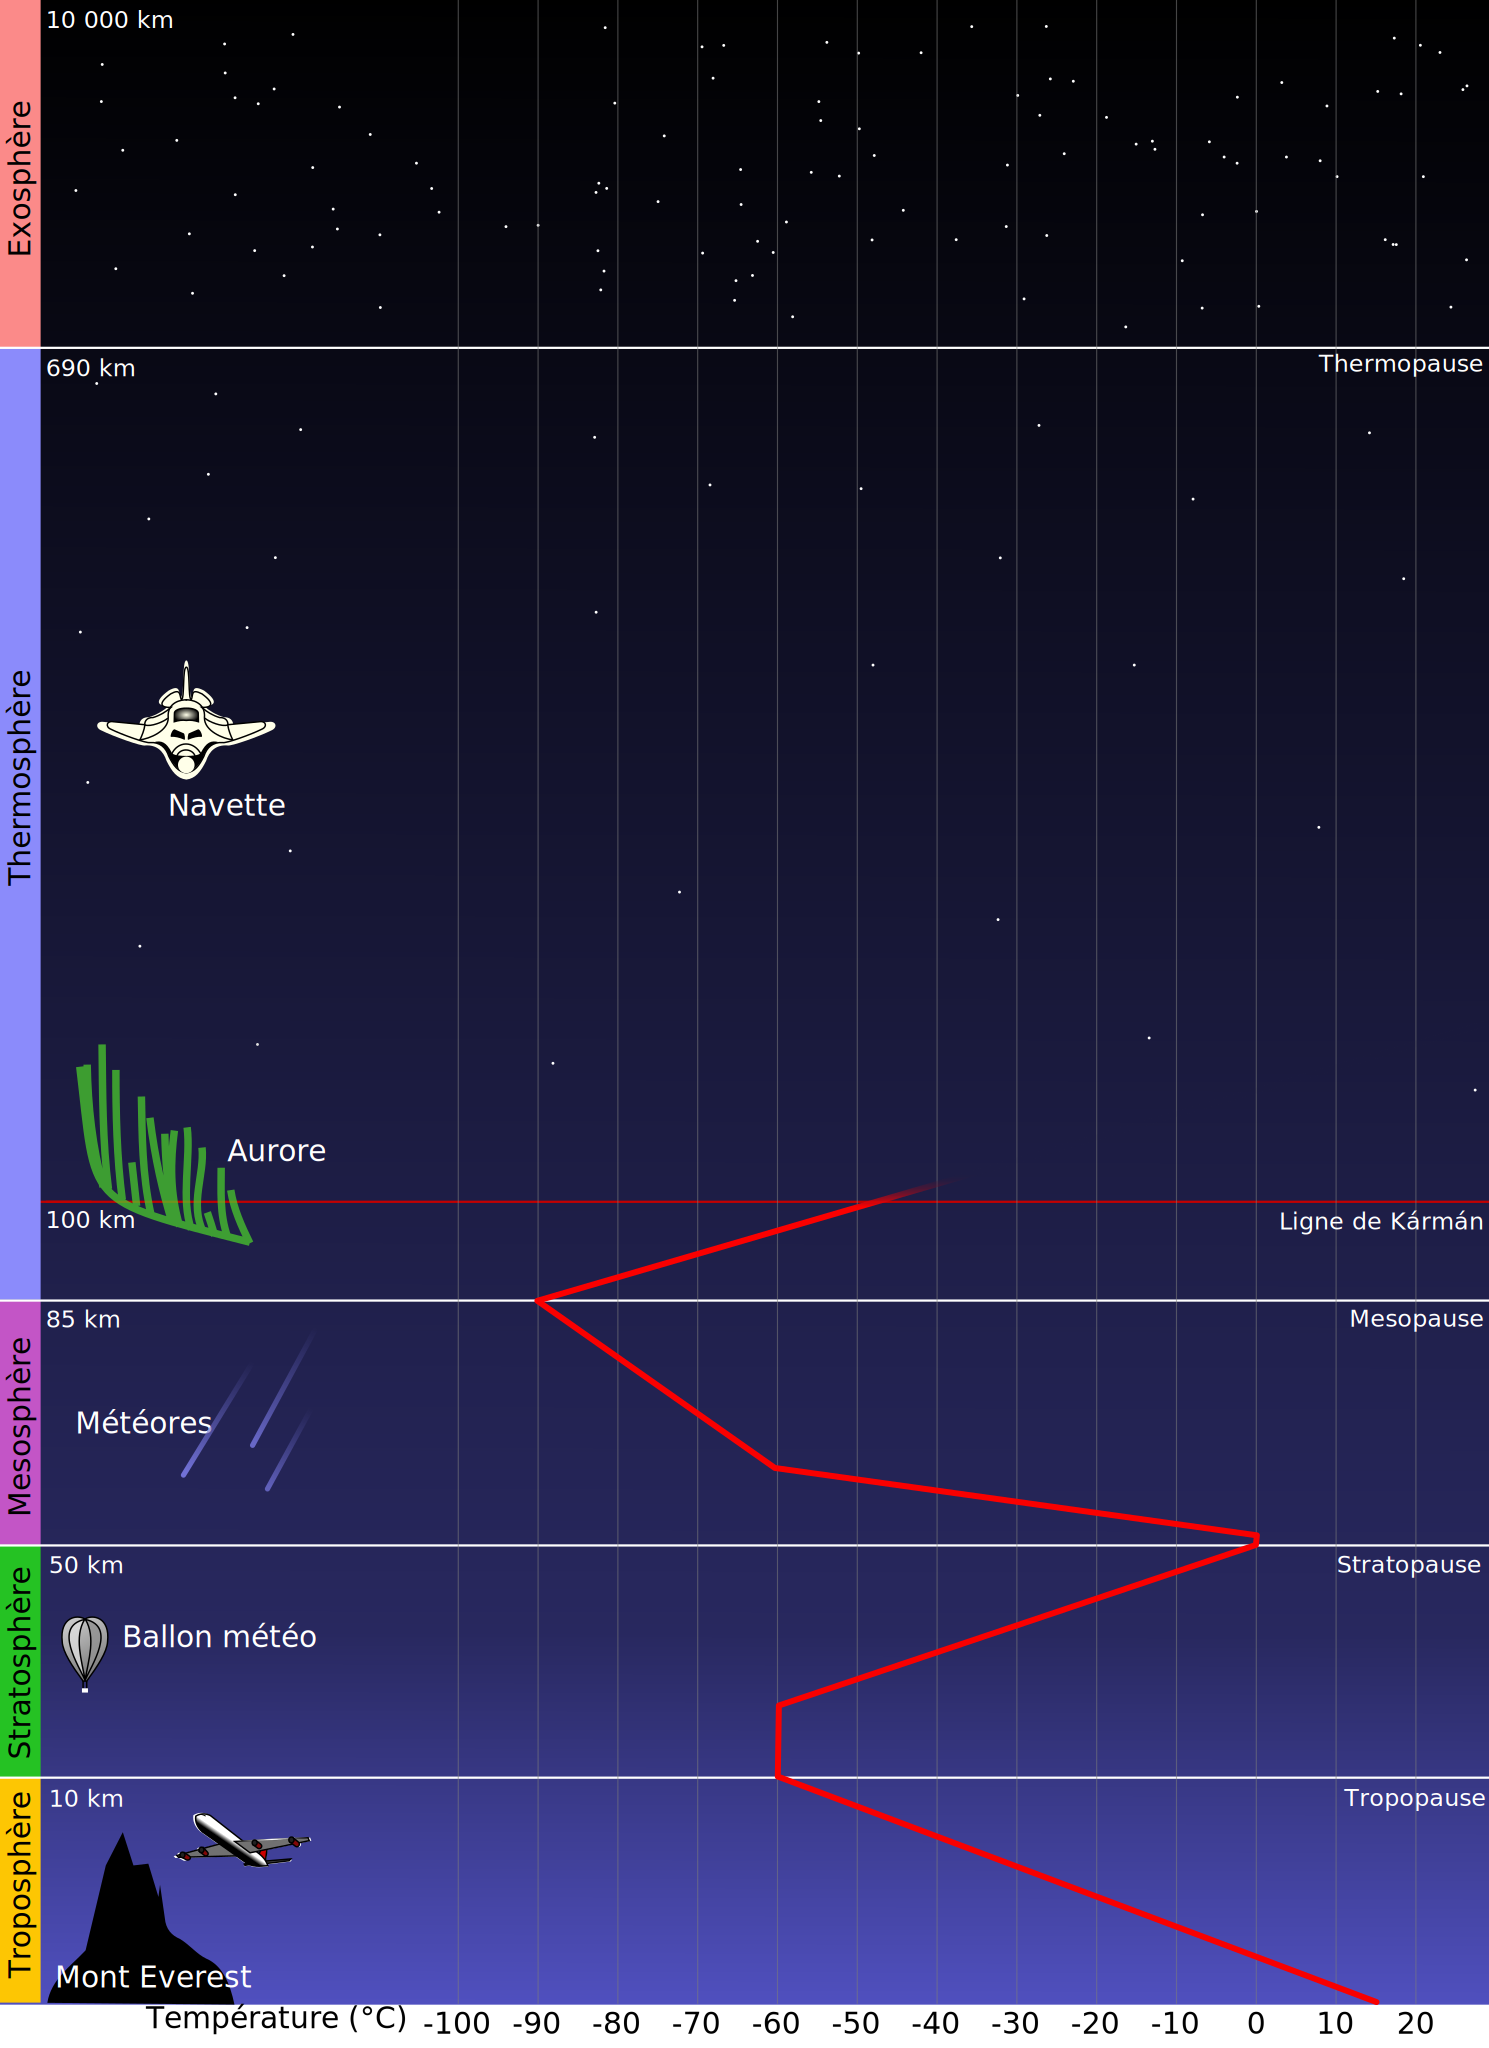
\includegraphics[width=0.38\linewidth]{03-Meteo/img/couchesAtmosphereTemperature.pdf}
			\legende{Schéma des couches de l'atmosphère}{img:couchesAtmosphereTemperature}
			\end{figure}	
	\end{frame}	
	
	\begin{frame}{La pression atmosphérique}
	
	\end{frame}
	
	\begin{frame}{L'atmosphère standard}
			On fixe les caractéristiques d'une atmosphère dite "standard" (ISA) comme suit :
			\begin{itemize}
				\item Température au niveau de la mer : $\ang{15}C$
				\item Pression atmosphérique au niveau de la mer : $1013,25~hPa$
			\end{itemize}
			
			Dans cette atmosphère standard, ces grandeurs évoluent comme ceci :
			\begin{itemize}
				\item $\ang{-0.65}C$ tous les $100~m$ (soit $\ang{-2}C$ tous les $1000~ft$), jusqu'à la tropopause
				\item $-1~hPa$ tous les $8,5~m$ (soit $-1~hPa$ tous les $28~ft$)
			\end{itemize}
	\end{frame}

 
\appendix 
\section{QCM}
\qmcBia{Étude des aéronefs}
{1}{Quels sont les éléments présents dans une commande de vol mécanique simple d'un avion d'aéroclub ?}
{Câbles et poulies}
{Tuyaux hydrauliques et servo-commande}
{Moteurs électriques et câbles}
{Bielles et pistons} 
{}
 
\ifdefined\activerbibliobeamer
\begin{frame}[allowframebreaks]
\frametitle{Bibliographie}
\printbibliography
%\nocite{*}
\end{frame}
\fi 
 
\end{document}
